After computing the matrix \(U\in \mathbb{R}^{N\times3}\) for both the \texttt{circle} and the \texttt{spiral} datasets and for each \(K \in \{10, 20, 40\}\) we can now finally deploy a clustering algorithm.
\\
\\
Let \(y_i\in \mathbb{R}^M\) be the vector corresponding to the \(i\)-th row of the matrix \(U\). Then we can use the \textit{K-Means} algorithm to cluster the points \(y_i\), \(i \in \{1, \dots, N\}\) into \(M\) clusters and assign the original datapoints to the same cluster as their corresponding rows in \(U\). 
\\
\\
The following code was used in order to perform clustering:
\lstinputlisting{../task6_7_8.m}
Hence for both dataset we obtain 3 different clusterings, one for each value of \(K\) tested. Plotting the results we obtain:
\begin{figure}[H]
    \centering
    \subfloat[1][\(K= 10\)]{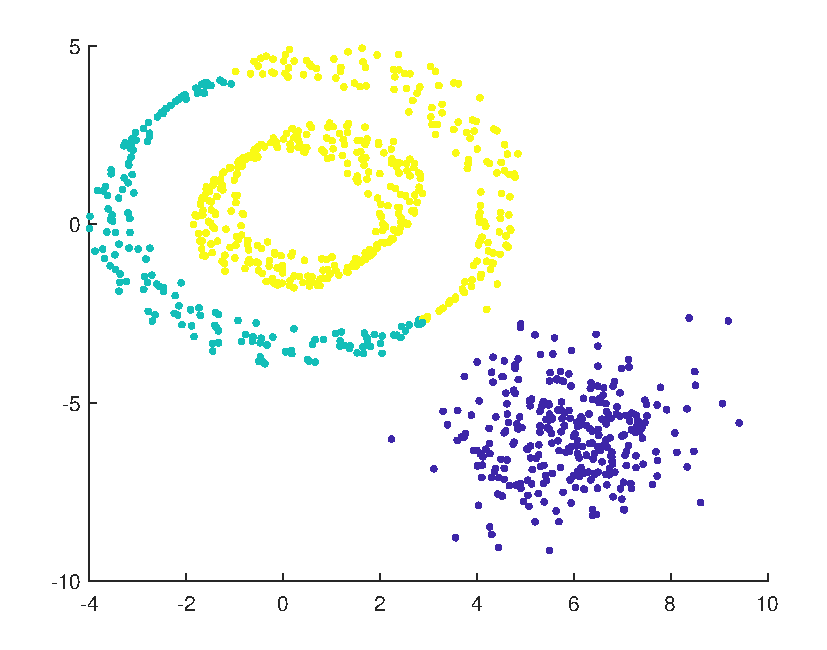
\includegraphics[scale = 0.37]{pictures/circle_SpectralClustering_K10.pdf}}
    \subfloat[2][\(K= 20\)]{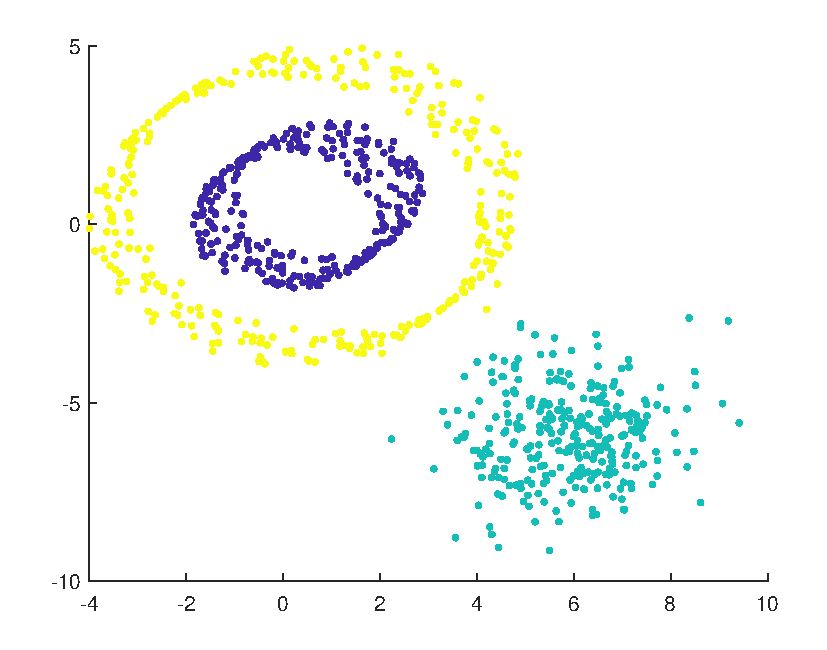
\includegraphics[scale = 0.37]{pictures/circle_SpectralClustering_K20.pdf}}
    \subfloat[3][\(K= 40\)]{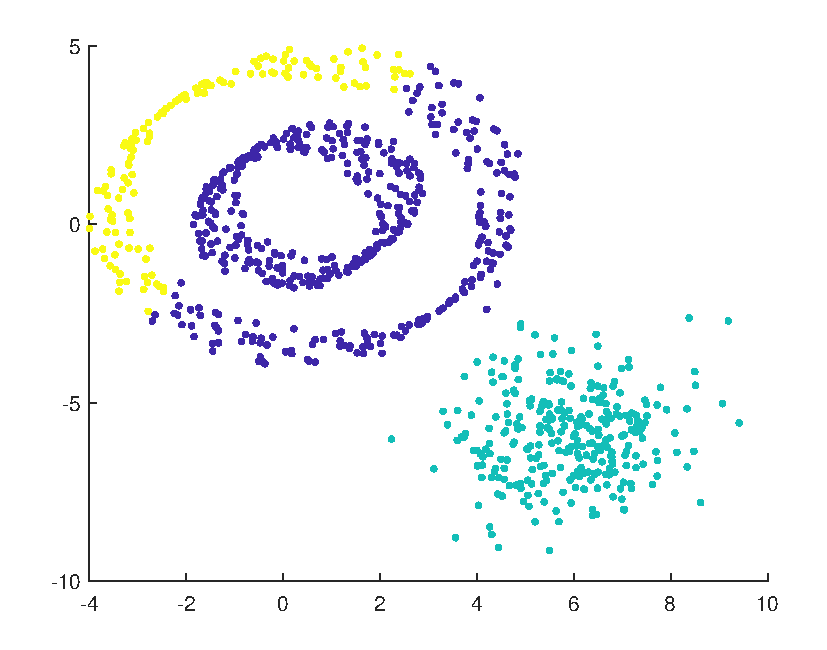
\includegraphics[scale = 0.37]{pictures/circle_SpectralClustering_K40.pdf}}
    \caption{Spectral clustering for \texttt{circle} data with different values of \(K\)}
    \label{spectral_circle}
  \end{figure}
  \begin{figure}[H]
    \centering
    \subfloat[1][\(K= 10\)]{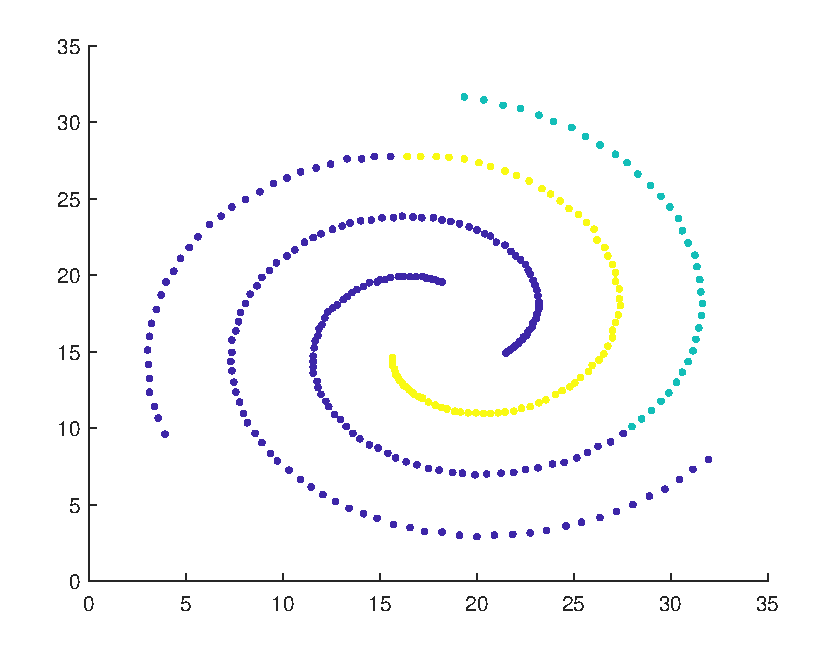
\includegraphics[scale = 0.37]{pictures/spiral_SpectralClustering_K10.pdf}}
    \subfloat[2][\(K= 20\)]{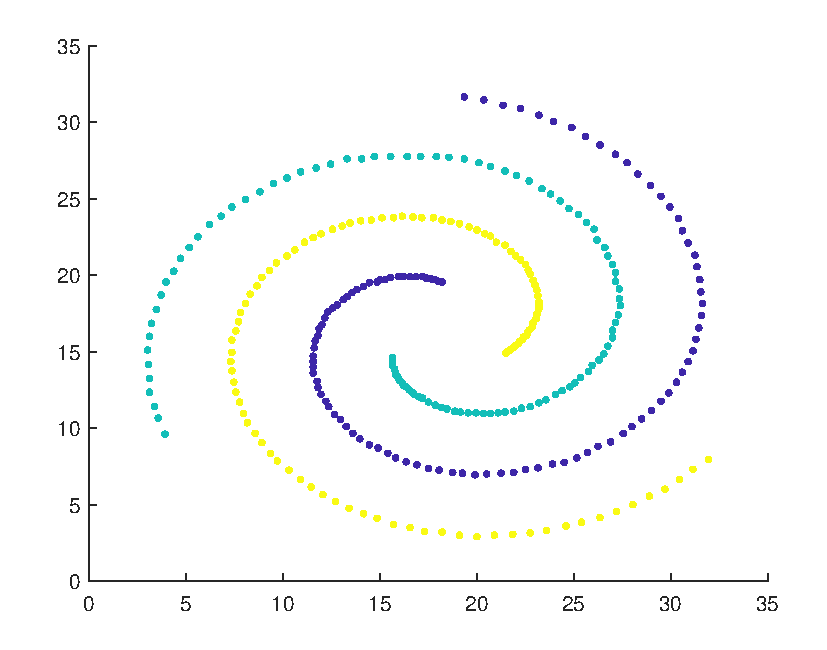
\includegraphics[scale = 0.37]{pictures/spiral_SpectralClustering_K20.pdf}}
    \subfloat[3][\(K= 40\)]{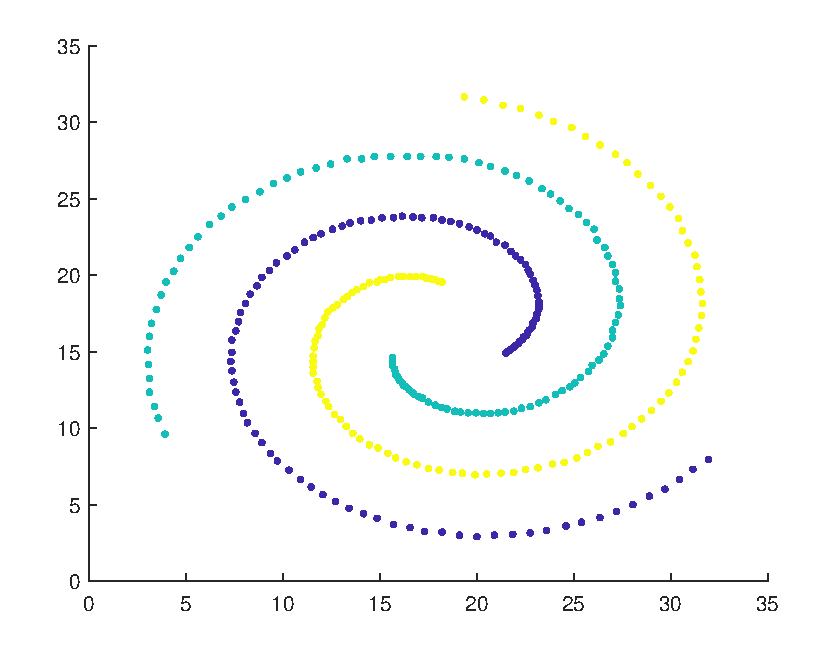
\includegraphics[scale = 0.37]{pictures/spiral_SpectralClustering_K40.pdf}}
    \caption{Spectral clustering for \texttt{spiral} data with different values of \(K\)}
    \label{spectral_spiral}
  \end{figure}
  \noindent As it is clearly visible in Figure \ref{spectral_circle}, performing spectral clustering on the \texttt{circle} data yields good results both in the case with \(K=10\) and \(K=20\). The same couldn't be said about the case \(K=40\) where the effect of pollution from one shape to another leads to poor results in terms of the proficiency of the algorithm to distinguish shapes.
  \\
  \\
  Although not every value of \(K\) yields good results for the \texttt{circle} data, the same isn't true for the \texttt{Spiral} data, where the presence of edges between spirals in the adjacency graph seems to have no effects on the fitness of the clustering, even with \(K=40\).